\documentclass{beamer}
% \usepackage{beamerthemesplit}
\usepackage{ragged2e}
\usepackage{CJKutf8}
\usepackage{tikz}
\usepackage{algorithm}
\usepackage{algorithmic}
\setbeamertemplate{theorems}[numbered]
\usepackage{clrscode3e}
\usepackage{mathrsfs}

\justifying\let\raggedright\justifying

\newtheorem{Exercise}{习题}

\begin{document}
\begin{CJK*}{UTF8}{gbsn}

\newtheorem{Thm}{定理}[section]
\newtheorem{Cor}{推论}[section]
\theoremstyle{definition}
\newtheorem{Def}{定义}[section]
\theoremstyle{example}
\newtheorem{Ex}{例}[section]
\date{}
\author{陈建文}

\title{第三章 关系}
\begin{frame}
  \titlepage
\end{frame}  
\section{关系的概念}
\begin{frame}
  \frametitle{1. 关系的概念}
  
  \begin{Def}\justifying\let\raggedright\justifying
    设$A$与$B$为两个集合。一个从$A\times B$到$\{T,F\}$的映射$R$,称为从$A$到$B$的一个\alert{二元关系}。
    $\forall (a,b) \in A \times B$,如果$(a,b)$在$R$下的象为$T$,则称$a$与$b$符合关系$R$,记为$aRb$;
    如果(a,b)在$R$下的象为$F$,则称$a$与$b$不符合关系$R$,记为$aR\!\!\! / b$。如
    果$A=B$,则称$R$为$A$上的二元关系。
  \end{Def}
  \pause
  \begin{Ex}
  设集合$X=\{1,2\}$,则$2^X$上的二元关系$\subseteq$可以定义为一个从$2^X\times
  2^X$到$\{T,F\}$的映射,

  $\subseteq(\{\phi\},\{\phi\})=T,\subseteq(\{\phi\},\{1\})=T,\subseteq(\{\phi\},\{2\})=T,\subseteq(\{\phi\},\{1,2\})=T,$

    $\subseteq(\{1\},\{\phi\})=F,\subseteq(\{1\},\{1\})=T,\subseteq(\{1\},\{2\})=F,\subseteq(\{1\},\{1,2\})=T,$

      $\subseteq(\{2\},\{\phi\})=F,\subseteq(\{2\},\{1\})=F,\subseteq(\{2\},\{2\})=T,\subseteq(\{2\},\{1,2\})=T,$

        $\subseteq(\{1,2\},\{\phi\})=F,\subseteq(\{1,2\},\{1\})=F,\subseteq(\{1,2\},\{2\})=F,\subseteq(\{1,2\},\{1,2\})=T$
\end{Ex}
\end{frame}
\begin{frame}
    \frametitle{1. 关系的概念}

  \begin{Def}\justifying\let\raggedright\justifying
    设$A$与$B$为两个集合。$A\times B$的任一子集$R$称为从$A$到$B$的一个\alert{二元关系}。如果$(a,b)\in R$,则称$a$与$b$符合关系$R$,记为$aRb$;如果$(a,b) \notin R$,则称$a$与$b$不符合关系$R$,并记为$aR\!\!\! / b$。
    如果$A=B$,则称$R$为$A$上的二元关系。
  \end{Def}\pause
    \begin{Ex}
  设集合$X=\{1,2\}$,则$2^X$上的二元关系$\subseteq$可以定义为$2^X\times
  2^X$的一个子集,

  \begin{equation*}
    \begin{split}
 \subseteq =& \{
 (\{\phi\},\{\phi\}),(\{\phi\},\{1\}),(\{\phi\},\{2\}),(\{\phi\},\{1,2\}),\\
 &(\{1\},\{1\}),(\{1\},\{1,2\}),
 (\{2\},\{2\}),(\{2\},\{1,2\}),\\&(\{1,2\},\{1,2\})
\}
    \end{split}
  \end{equation*}
\end{Ex}

\end{frame}

\begin{frame}
  \frametitle{1. 关系的概念}
  \begin{Ex}
    自然数集$\mathbb{N}$上的小于等于关系"$\leq$"是$\mathbb{N}$上的一个二元关系。
  \end{Ex}\pause
  \begin{Ex}\justifying\let\raggedright\justifying
    设$n$为任一给定的自然数。对任意的两个整数$m$,$k$,如果$m-k$能被$n$整除,则称$m$与$k$为模$n$同余,并记为$m\equiv k \pmod{n}$。
    显然,$m\equiv k \pmod{n}$当且仅当$m$被$n$除所得到的余数与$k$被$n$除所得到的余数相等。模$n$同余是$\mathbb{Z}$上的一个二元关系。
  \end{Ex}
\end{frame}

\begin{frame}
  \frametitle{1. 关系的概念}
  \begin{Def}
    设$R \subseteq A \times B$,集合
    \[\{x \in A | \exists y \in B \text{使得} (x,y) \in R\}\]
    称为$R$的\alert{定义域},记为$dom(R)$; 集合
    \[\{y \in B | \exists x \in A \text{使得} (x,y) \in R\}\]
    称为$R$的\alert{值域},记为$ran(R)$。
  \end{Def}
\end{frame}



\begin{frame}
  \frametitle{1. 关系的概念}
  \begin{Def}
    设$A_1, A_2, \ldots, A_n$为$n$个集合,一个$A_1\times A_2 \times \cdots \times A_n$的子集$R$称为$A_1, A_2, \cdots, A_n$间的一个\alert{$n$元关系},每个$A_i$称为$R$的一个域。
  \end{Def}
\end{frame}
\section{关系的性质}
\begin{frame}
  \frametitle{2. 关系的性质}
  \begin{Def}
    集合$X$上的二元关系$R$称为\alert{自反}的,如果对$X$的任意元素$x$都有$xRx$。
  \end{Def}
  \pause
    判断下列二元关系是否是自反的。设集合$X=\{1,2,3,4\}$,
  \begin{enumerate}
  \item 集合$X$上的二元关系$R=\{(1,2), (1,3), (1,4), (2,3),
    (2,4), (3,4)\}$
  \item 集合$X$上的二元关系$R=\{(1,1), (1,2), (2,2),
    (2,4), (3,3), (4,4)\}$
  \item 集合$X$上的二元关系$R = \{(1,1), (2,3), (3,2)\}$
  \item 集合$X$上的二元关系$R = \{(2,3)\}$
  \item 集合$X$上的恒等关系$I_X = \{(1,1), (2,2), (3,3),(4,4)\}$
%  \item 设集合$X = \{0,1\}$, $2^X$上的二元关系$\subseteq$
  \end{enumerate}

\end{frame}

\begin{frame}
  \frametitle{2. 关系的性质}
  \begin{Def}
   集合$X$上的二元关系$R$称为\alert{反自反}的,如果对$X$的任意元素$x$都有$(x,x) \notin R$。
 \end{Def}
   \pause
    判断下列二元关系是否是反自反的。设集合$X=\{1,2,3,4\}$,
  \begin{enumerate}
  \item 集合$X$上的二元关系$R=\{(1,2), (1,3), (1,4), (2,3),
    (2,4), (3,4)\}$
  \item 集合$X$上的二元关系$R=\{(1,1), (1,2), (2,2),
    (2,4), (3,3), (4,4)\}$
  \item 集合$X$上的二元关系$R = \{(1,1), (2,3), (3,2)\}$
  \item 集合$X$上的二元关系$R = \{(2,3)\}$
  \item 集合$X$上的恒等关系$I_X = \{(1,1), (2,2), (3,3),(4,4)\}$
%  \item 设集合$X = \{0,1\}$, $2^X$上的二元关系$\subseteq$
  \end{enumerate}
\end{frame}
\begin{frame}
  \frametitle{2. 关系的性质}
  \begin{Def}
    集合$X$上的二元关系$R$称为\alert{对称}的,如果对$X$的任意元素$x$,$y$,只要$xRy$就有$yRx$。
  \end{Def}
    \pause
    判断下列二元关系是否是对称的。设集合$X=\{1,2,3,4\}$,
  \begin{enumerate}
  \item 集合$X$上的二元关系$R=\{(1,2), (1,3), (1,4), (2,3),
    (2,4), (3,4)\}$
  \item 集合$X$上的二元关系$R=\{(1,1), (1,2), (2,2),
    (2,4), (3,3), (4,4)\}$
  \item 集合$X$上的二元关系$R = \{(1,1), (2,3), (3,2)\}$
  \item 集合$X$上的二元关系$R = \{(2,3)\}$
  \item 集合$X$上的恒等关系$I_X = \{(1,1), (2,2), (3,3),(4,4)\}$
%  \item 设集合$X = \{0,1\}$, $2^X$上的二元关系$\subseteq$
  \end{enumerate}
\end{frame}
\begin{frame}
  \frametitle{2. 关系的性质}
  \begin{Def}
         集合$X$上的二元关系$R$称为\alert{反对称}的,如果对$X$的任意元素$x$,$y$,$xRy$且$yRx$,则$x=y$。    
       \end{Def}
         \pause
    判断下列二元关系是否是反对称的。设集合$X=\{1,2,3,4\}$,
  \begin{enumerate}
  \item 集合$X$上的二元关系$R=\{(1,2), (1,3), (1,4), (2,3),
    (2,4), (3,4)\}$
  \item 集合$X$上的二元关系$R=\{(1,1), (1,2), (2,2),
    (2,4), (3,3), (4,4)\}$
  \item 集合$X$上的二元关系$R = \{(1,1), (2,3), (3,2)\}$
  \item 集合$X$上的二元关系$R = \{(2,3)\}$
  \item 集合$X$上的恒等关系$I_X = \{(1,1), (2,2), (3,3),(4,4)\}$
%  \item 设集合$X = \{0,1\}$, $2^X$上的二元关系$\subseteq$
  \end{enumerate}
\end{frame}
\begin{frame}
  \frametitle{2. 关系的性质}
  \begin{Def}
        集合$X$上的二元关系$R$称为\alert{传递}的,如果对$X$的任意元素$x$,$y$,$z$,只要$xRy$且$yRz$,就有$xRz$。
      \end{Def}
        \pause
    判断下列二元关系是否是传递的。设集合$X=\{1,2,3,4\}$,
  \begin{enumerate}
  \item 集合$X$上的二元关系$R=\{(1,2), (1,3), (1,4), (2,3),
    (2,4), (3,4)\}$
  \item 集合$X$上的二元关系$R=\{(1,1), (1,2), (2,2),
    (2,4), (3,3), (4,4)\}$
  \item 集合$X$上的二元关系$R = \{(1,1), (2,3), (3,2)\}$
  \item 集合$X$上的二元关系$R = \{(2,3)\}$
  \item 集合$X$上的恒等关系$I_X = \{(1,1), (2,2), (3,3),(4,4)\}$
%  \item 设集合$X = \{0,1\}$, $2^X$上的二元关系$\subseteq$
  \end{enumerate}
\end{frame}
\section{关系的运算}
\begin{frame}
  \frametitle{3. 关系的运算}
  \begin{Def}
    设$R$为从集合$A$到集合$B$的二元关系,$R$的\alert{逆}$R^{-1}$定义为从集合$B$
    到集合$A$的二元关系
    \[R^{-1}=\{(y,x)|(x,y)\in R\}\]
  \end{Def}\pause
  \begin{Thm}
    设$R$为集合$X$上的二元关系,则$R$为对称的当且仅当$R=R^{-1}$。
  \end{Thm}  
\end{frame}
\begin{frame}
  \frametitle{3. 关系的运算}
  \begin{Def}\justifying\let\raggedright\justifying
    设$R$为从集合$A$到集合$B$,$S$为从集合$B$到集合$C$的二元关系。$R$与$S$的合成
    $R\circ S$定义为从集合$A$到集合$C$的一个二元关系
    \[R\circ S = \{(x,z)\in A \times C |  \exists y \in B \text{使得} xRy \text{且} ySz\}\]
  \end{Def}\pause
    \begin{Thm}
    设$R_1$,$R_2$,$R_3$分别为从集合$A$到集合$B$,从集合$B$到集合$C$,从集合$C$到集合$D$的二元关系,则
    \[(R_1 \circ R_2)\circ R_3 = R_1 \circ (R_2 \circ R_3)\]
  \end{Thm}\pause
  \begin{Thm}
    设$R$为集合$X$上的一个二元关系,则$R$为传递的当且仅当$R\circ R \subseteq R$。
  \end{Thm}\pause
\end{frame}

\section{关系矩阵}
\begin{frame}
  \frametitle{4. 关系矩阵和关系图}
  \begin{Def}\justifying\let\raggedright\justifying
    设$X=\{x_1, x_2, \ldots, x_m\}$为一个包含$m$个元素的集合,$Y=\{y_1, y_2,
    \cdots, y_n\}$为一个包含$n$个元素的集合。令$R$是从$X$到$Y$的一个二元关系。
    由$R$定义一个$m \times n$矩阵$B = (b_{ij})$如下: $\forall (x_i, y_j) \in X \times Y$,
\[
    b_{ij}=
      \begin{cases}
        1,&\text{如果}x_iRy_j\\
        0,&\text{如果}x_iR\!\!\! / y_j
      \end{cases}
\]
    则矩阵$B$称为关系$R$的矩阵。
  \end{Def}
\end{frame}
\begin{frame}
  \frametitle{4. 关系矩阵和关系图}
  \begin{Ex}
    设$X=\{1,2,3,4\}$,$Y=\{a, b, c, d, e\}$, 从$X$到$Y$的关系$S=\{(1,a),  (2, b), (2, d), (2, e), (3, a), (3, b), (3, d),  (3, e), (4,c), (4,d)\}$,则$S$的关系矩阵为?
  \end{Ex}
  \pause
  \begin{Ex}
    设$X = \{1,2,3,4\}$,$R = \{(1,1),(1,2),(1,3),(1,4),(2,2),(2,4),(3,3),(4,2),(4,4)\}$,则$R$的关系矩阵为?
  \end{Ex}
\end{frame}
\begin{frame}
  \frametitle{4. 关系矩阵和关系图}
  \begin{Thm}
  设$B$为集合$X$上二元关系$R$的矩阵,则
  \begin{enumerate}[(1)]
  \item $R$为自反的,当且仅当$B$的对角线上的全部元素都为1;
  \item $R$为反自反的,当且仅当$B$的对角线上的全部元素都为0;
  \item $R$为对称的,当且仅当$B$是对称矩阵;
  \item $R$为反对称的,当且仅当$i \neq j$时$b_{ij}$与$b_{ji}$不同时为1;
  \item $R$为传递的,当且仅当如果$b_{ij}=1$且$b_{jk}=1$,则$b_{ik}=1$。
  \end{enumerate}
\end{Thm}
\end{frame}
\begin{frame}
  \frametitle{4. 关系矩阵和关系图}
  \begin{Thm}
  设$R$为集合$X$上的二元关系,则
  \begin{enumerate}[(1)]
  \item $R$是自反的,当且仅当$R$的图的每个顶点均有一个环;
  \item $R$是反自反的,当且仅当$R$的图中没有环;
  \item $R$是对称的,当且仅当$R$的图中任意两个不同顶点间有矢线,则必有两条方向相反的矢线;
  \item $R$是反对称的,当且仅当$R$的图中任意两个不同顶点间有矢线,则不能有两条方向相反的矢线;
  \item $R$是传递的,当且仅当如果从某顶点沿矢线经两条矢线可到另一顶点,则从该顶点到另一顶点有一条矢线。
  \end{enumerate}
\end{Thm}
\end{frame}
\begin{frame}
  \frametitle{4. 关系矩阵和关系图}
  \begin{Thm}
    设$B$为集合$X$上二元关系$R$的矩阵,则$R^{-1}$的矩阵为$B^{T}$。
  \end{Thm}
\end{frame}

\begin{frame}
  \frametitle{4. 关系矩阵和关系图}
  \begin{Def}
    设$B$,$C$是两个布尔矩阵,$B$与$C$的逻辑乘为$B$与$C$的对应元素进行逻辑乘,所得到的布尔矩阵记为$B \land C$,即
    \begin{equation*}
      B \land C = (b_{ij} \land c_{ij})
    \end{equation*}
    $B$与$C$的逻辑加为$B$与$C$的对应元素进行逻辑加,所得到的布尔矩阵记为$B \lor C$,即
    \begin{equation*}
      B \lor C = (b_{ij} \lor c_{ij})
    \end{equation*}
  \end{Def}
  \begin{Thm}
    设$R$,$S$为从集合$X$到集合$Y$的二元关系,其矩阵分别为$B_R$和$B_S$。 $R\cup S$ 与$R \cap S$的矩阵分别为$B_{R\cup S}$,$B_{R\cap S}$,则
    \begin{equation*}
      B_{R\cup S}=B_R \lor B_S, B_{R\cap S}=B_R \land B_S
    \end{equation*}
  \end{Thm}
\end{frame}

\begin{frame}
  \frametitle{4. 关系矩阵和关系图}
  \begin{Def}
    设$A$为$m\times p$布尔矩阵,$B$为$p \times n$布尔矩阵,$A$与$B$的布尔乘积$A \circ B$定义为矩阵$C$,其元素计算如下
    \begin{align*}
      c_{ij} &= (a_{i1}\land b_{1j}) \lor (a_{i2} \land b_{2j}) \lor \cdots \lor (a_{ip} \land b_{pj}), \\
      i &= 1,2,\cdots, m, j = 1,2,\cdots, n
    \end{align*}
  \end{Def}\pause
  \begin{Thm}
    设$X, Y, Z$为有穷集合, $|X| =m$,$|Y|=p$,$|Z| = n$。$R$为从$X$到$Y$的二元
    关系, $S$为从$Y$到$Z$的二元关系,$R$,$S$,$R \circ S$的矩阵分别为$B_{R}$,$B_{S}$,$B_{R\circ S}$,则$B_{R\circ S} = B_R \circ B_S$。
  \end{Thm}
\end{frame}

\section{关系的闭包}
\begin{frame}
  \frametitle{5. 关系的闭包}
  \begin{Def}
    设$R$为集合$X$上的一个二元关系。$X$上的一切包含$R$的传递关系的交称为$R$的传递闭包,用$R^+$表示。即
    \begin{equation*}
      R^+ = \bigcap_{R \subseteq R' \text{且} R'\text{是传递的}}R'
    \end{equation*}
  \end{Def}
  \pause
  \begin{Thm}
    设$R$为集合X上的一个二元关系,则关系$R$的传递闭包$R^+$为包含$R$的传递关系。
  \end{Thm}
\end{frame}
\begin{frame}
  \frametitle{5. 关系的闭包}
  \begin{Thm}
    设$R$为集合$X$上的一个二元关系,$a \in X$,$b \in X$,$n \geq 2$,则$(a,b) \in R^n$当且仅当存在$x_1\in X$,$x_2\in X$,$\ldots$,$x_{n-1}\in X$,使得$(a, x_1) \in R$,$(x_1, x_2)\in R$,  $\ldots$, $(x_{n-1}, b)\in R$。
  \end{Thm}
  \begin{proof}[证明]
  \pause 用数学归纳法证明,施归纳于$n$:

  \pause 当$n=2$时,由关系合成运算的定义知$(a,b)\in R^2$当且仅当存在$x_1\in X$使得$(a,x_1)\in R$且$(x_1, b)\in R$,结论成立。

  \pause 假设当$n=k$时定理的结论成立,往证当$n=k+1$时定理的结论也成立。
  \pause 由关系合成运算的定义知$(a,b)\in R^{k+1}$当且仅当存在\\$x\in X$使得$(a,x)\in R^k$且$(x, b)\in R$。\pause 由归纳假设,$(a,x)\in R^k$当且仅当存在$x_1\in X$,$x_2\in X$,$\ldots$,$x_{k-1}\in X$,使得$(a, x_1) \in R$,\\ $(x_1, x_2)\in R$,  $\ldots$, $(x_{k-1}, x)\in R$。\pause 记$x_{k}=x$,则$(a,b)\in R^{k+1}$当且仅当存在$x_1\in X$,$x_2\in X$,$\ldots$,$x_{k-1}\in X$,$x_{k}\in X$,使得\\$(a, x_1) \in R,(x_1, x_2)\in R,\ldots,(x_{k-1}, x_k)\in R,(x_k, b)\in R$。
\end{proof}

\end{frame}
\begin{frame}
  \frametitle{5. 关系的闭包}
  \begin{Thm}
    设$R$为集合$X$上的一个二元关系,则
    \begin{equation*}
      R^+ = \bigcup_{n=1}^\infty R^n = R \cup R^2 \cup R^3 \cup \cdots 
    \end{equation*}
  \end{Thm}
\end{frame}
\begin{frame}
  \frametitle{5. 关系的闭包}
  \begin{Thm}
    设$R$为集合$X$上的一个二元关系,$|X| = n$,则\[R^+ = \bigcup_{i=1}^nR^i = R \cup R^2  \cup \cdots \cup R^n \]。
  \end{Thm}
  \begin{proof}[证明]\justifying\let\raggedright\justifying\small{
      只须证明对任一自然数$k > n$,有$R^k \subseteq \bigcup_{i=1}^nR^i$。\pause
      为此,设$(a,b) \in R^k$,则存在$b_1, b_2, \cdots, b_{k-1} \in
      X$使得$(a,b_1) \in R$, $(b_1, b_2) \in R, \cdots, (b_{k-2}, b_{k-1})\in R,
      (b_{k-1}, b) \in R$。记$b_0 = a, b_k = b$。 \pause $b_1,b_2, \cdots,
      b_{k-1}, b$是$X$中的$k$个元素,而$X$中仅有$n$个元素,$n < k$,所以$b_1,
      b_2, \cdots, b_{k-1}, b$中必有两个相等的元素。设$b_i=b_j$,$1 \leq i < j
      \leq k$。 \pause 于是,我们有$(a,b_1)\in R, \cdots, (b_{i-1}, b_i)\in R,
      (b_j, b_{j+1})\in R, \cdots, (b_{k-1},b)\in R$,故$(a,b)\in
      R^{k-(j-i)}$,$p_1=k-(j-i) < k$。 \pause 若$p_1 = k - (j - i) > n$, 则重复
      上述过程又有$p_2 < p_1$使得$(a,b) \in R^{p_2}$。 \pause 如此进行下去,必
      有$m \leq n$使得$(a,b) \in R^m$。所以,$R^k \subseteq
      \bigcup_{i=1}^nR^i$。 \pause 因此,$R^+=\bigcup_{i=1}^nR^i$。}
  \end{proof}
\end{frame}
\begin{frame}
  \frametitle{5. 关系的闭包}
  \begin{Thm}
    设$R$为集合$X$上的一个二元关系,$|X| = n$, $B$为$R$的关系矩阵,$B_{R^+}$为$R^+$的关系矩阵,简记为$B^+$,则
    \begin{equation*}
      B^+ = B \lor B^{(2)} \lor \cdots \lor B^{(n)}
    \end{equation*}
  \end{Thm}
\end{frame}

\begin{frame}
  \frametitle{5. 关系的闭包}
  \begin{codebox}
    \Procname{$\proc{Transitive-Closure}(B)$}
    \zi \Comment $B$ is the zero-one $n \times n$ matrix for relation $R$
    \li $M \gets B$
    \li $A \gets M$
    \li \For $i \gets 2$ \To $n$
    \li \Do
        $M \gets M \circ B$
    \li $A \gets A \lor M$
    \End
    \li \Return A \Comment $A$ is the zero-one matrix for $R^+$
  \end{codebox}
  
\end{frame}

\begin{frame}
  \frametitle{5. 关系的闭包}
  \begin{codebox}
    \Procname{$\proc{Warshall}(B)$}
    \zi \Comment $B$ is the zero-one $n \times n$ matrix for relation $R$
    \li $A \gets B$
    \li \For $k \gets 1$ \To $n$
    \li \Do
    \For $i \gets 1$ \To $n$
    \li \Do
    \For $j \gets 1$ \To $n$
    \li \Do
    $a_{ij} = a_{ij} \lor (a_{ik} \land a_{kj})$
    \End
    \End
    \End
    \li \Return A \Comment $A$ is the zero-one matrix for $R^+$
  \end{codebox}  
\end{frame}

\begin{frame}
  \frametitle{5. 关系的闭包}
  \begin{codebox}
    \Procname{$\proc{Warshall}(B)$}
    \zi \Comment $B$ is the zero-one $n \times n$ matrix for relation $R$
    \li $A \gets B$
    \li \For $k \gets 1$ \To $n$
    \li \Do
    \For $i \gets 1$ \To $n$
    \li \Do
     \If $a_{ik} \isequal 1$
    \li \Then
    \For $j \gets 1$ \To $n$
    \li \Do
    $a_{ij} = a_{ij} \lor (a_{ik} \land a_{kj})$
    \End
    \End
    \End
    \End
    \li \Return A \Comment $A$ is the zero-one matrix for $R^+$
  \end{codebox}  
\end{frame}

% \begin{frame}[fragile]
%   \frametitle{4. 关系的闭包}
%   \begin{algorithm}[H]
%     \caption{Computing the Transitive Closure}
%     \begin{algorithmic}
%     \REQUIRE $M_R$: zero-one $n \times n$ matrix for relation $R$
%     \ENSURE $B$: zero-one $n \times n$ matrix for realtion $R^*$
%      \STATE $A \leftarrow M_R$
%      \STATE $B \leftarrow A$      
%     \end{algorithmic}
%   \end{algorithm}
% \end{frame}

\section{等价关系与集合的划分}
\begin{frame}
  \frametitle{6. 等价关系与集合的划分}
  \begin{Def}
    集合$X$上的二元关系$R$称为\alert{等价关系},如果$R$同时满足以下三个性质:
    \begin{enumerate}[(1)]
    \item $R$是自反的,即对$X$中的任意元素$x$,$xRx$;
    \item $R$是对称的,即对$X$中的任意元素$x$,$y$,如果$xRy$,则$yRx$;
    \item $R$是传递的,即对$X$中的任意元素$x$,$y$,$z$,如果$xRy$且$yRz$,则$xRz$。
    \end{enumerate}
  \end{Def}
\end{frame}
\begin{frame}
  \frametitle{6. 等价关系与集合的划分}
  \begin{Ex}
    整数集$\mathbb{Z}$上的模$n$同余关系是$\mathbb{Z}$上的等价关系。
  \end{Ex}\pause
  \begin{Ex}
    设集合
    $X=\{1,2,3,4,5,6 \}$上的关系$R$定义如下:
    \begin{align*}
      R=&\{(1,1),(1,3),(1,5),(2,2),(2,4),(3,1),(3,3),(3,5),(4,2),\\
      &(4,4),(5,1),(5,3),(5,5),(6,6)\},
    \end{align*}
  \end{Ex}
  则$R$为$X$上的等价关系。
\end{frame}
\begin{frame}
  \frametitle{6. 等价关系与集合的划分}
  \begin{Def}
    设$\cong$为集合$X$上的一个等价关系,$x\in X$,$X$的子集
    \[E_x=\{y\in X | x \cong y\}\]称为$x$关于$\cong$的\alert{等价类},记为$[x]$,即
    \begin{equation*}
      [x] = \{y \in X | x \cong y\}
    \end{equation*}
  \end{Def}
\end{frame}
\begin{frame}
  \frametitle{6. 等价关系与集合的划分}
  \begin{Def}
    设$X$为集合, $X$的一些非空子集形成的集族$\mathscr{A}$称为$X$的一个划分,如果$\mathscr{A}$具有性质
    \begin{enumerate}
    \item $\forall A, B \in \mathscr{A}$,如果$A \neq B$,则$A \cap B = \phi$;
      \item $\bigcup_{A \in \mathscr{A}} = X$
    \end{enumerate}
  \end{Def}
\end{frame}

\begin{frame}
  \frametitle{6. 等价关系与集合的划分}
  \begin{Thm}
    设$\cong$为集合$X$上的一个等价关系,则$\cong$的所有等价类的集合构成$X$的一个划分。
  \end{Thm}
  \pause
  \begin{Thm}
    设$\mathscr{A}$为集合$X$的一个划分。令
    \begin{equation*}
      \cong = \bigcup_{A\in \mathscr{A}}A\times A
    \end{equation*}
    则$\cong$是$X$上的一个等价关系且$\mathscr{A}$就是$\cong$的等价类之集。
  \end{Thm}
\end{frame}
\begin{frame}
  \frametitle{6. 等价关系与集合的划分}
  \begin{Thm}
    设$X$为一个集合,
    \begin{align*}
    \mathbb{R} &= \{\cong \subseteq X \times X | \cong\text{为集合}X\text{上的一个等价关系}\},\\
      \mathbb{A} &= \{\mathscr{A} \subseteq 2^X| \mathscr{A}\text{为集合}X\text{的一个划分}\},\\
      f &= \{(\cong, \{[x]_{\cong} | x \in X\})|\cong \in \mathbb{R}, [x]_{\cong}=\{y\in X | x \cong y\}\}\\
      g&=\{(\mathscr{A}, \bigcup_{A \in \mathscr{A}}A\times A)|\mathscr{A} \in \mathbb{A}\}\\
    \end{align*}
    则$f$为从$\mathbb{R}$到$\mathbb{A}$的双射,且$f^{-1}=g$。
  \end{Thm}
  
\end{frame}

\begin{frame}
  \frametitle{6. 等价关系与集合的划分}
  \begin{proof}[证明]
    \begin{enumerate}
    \item 证明$f$为映射。这就是要证明对于集合$X$上的任意一个等价关系$\cong$, 
      $\{[x]_{\cong}|x\in X\}$为集合$X$的一个划分。
    \item 证明$g$为映射。这就是要证明对于集合$X$的任意一个划分$\mathscr{A}$,
      $\bigcup_{A\in \mathscr{A}}A\times A$为集合$X$上的一个等价关系。
    \item 证明$g\circ f = I_{\mathbb{R}}$。这就是要证明对于集合$X$上的任意一个等
      价关系$\cong$,$\bigcup_{x\in X}[x]_{\cong}\times [x]_{\cong} = \cong$。
    \item 证明$f\circ g = I_{\mathbb{A}}$。这就是要证明对于集合$X$上的任意一个划分
      $\mathscr{A}$,等价关系$\bigcup_{A \in \mathscr{A}}A\times A$所对应的等价类
      的集合就是$\mathscr{A}$。
    \end{enumerate}
  \end{proof}
  
\end{frame}

\section{偏序关系}
\begin{frame}
  \frametitle{7. 偏序关系与偏序集}
  \begin{Def}
    集合$X$上的二元关系$R$称为\alert{偏序关系},如果$R$同时满足以下三个性质:
    \begin{enumerate}[(1)]
    \item $R$是自反的,即对$X$中的任意元素$x$,$xRx$;
    \item $R$是反对称的,即对$X$中的任意元素$x$,$y$,如果$xRy$且$yRx$,则$x=y$;
    \item $R$是传递的,即对$X$中的任意元素$x$,$y$,$z$,如果$xRy$且$yRz$,则$xRz$。
    \end{enumerate}
  \end{Def}\pause
    \begin{Def}
    设$\leq$为集合$X$上的一个偏序关系,则称二元组$(X,\leq)$为\alert{偏序集}。
  \end{Def}
\end{frame}

\begin{frame}
  \frametitle{7. 偏序关系与偏序集}
  \begin{Ex}
    实数集$\mathbb{R}$上通常的“小于等于”关系$\leq$是偏序关系,所以$(\mathbb{R},\leq)$为偏序集。
  \end{Ex}
  \begin{Ex}
    设$S$为一个集合,$S$的子集间的包含关系$\subseteq$是$2^S$上的偏序关系,所以$(2^{\mathbb{S}},\subseteq)$为偏序集。
  \end{Ex}
\end{frame}

\begin{frame}
  \frametitle{7. 偏序关系与偏序集}
  \begin{Ex}
    设集合
    $X=\{a,b,c,d\}$上的关系$R$定义如下:
    \begin{equation*}
      R=\{(a,a),(a,b),(a,c),(a,d),(b,b),(b,d),(c,c),(c,d),(d,d)\}
    \end{equation*}
  \end{Ex}
  则$R$为$X$上的偏序关系。
\end{frame}

\begin{frame}
\frametitle{7. 偏序关系与偏序集}
  \begin{Def}\justifying\let\raggedright\justifying
    设$\leq$为集合$X$上的偏序关系,如果$\forall x, y \in X$,$x \leq y$与$y \leq x$至少有一个成立,则称$\leq$为$X$上的\alert{全序关系}。相应的,二元组$(X,\leq)$称为\alert{全序集}。
  \end{Def}
\end{frame}
\begin{frame}
  \frametitle{7. 偏序关系与偏序集}
  \begin{Def}
    设$(X,\leq)$为一个偏序集,$A\subseteq X$。如果存在一个元素$s\in A$使得$\forall x \in A$有$x \leq s$,则称$s$为$A$的\alert{最大元素};如果存在一个元素$t\in A$使得$\forall x \in A$有$t \leq x$,则称$t$为$A$的\alert{最小元素}。
  \end{Def}
    \begin{Def}
    设$(X,\leq)$为一个偏序集,$A\subseteq X$。如果存在一个元素$s\in A$,在$A$中没
    有元素$x$使得$s < x$,则称$s$为$A$的\alert{极大元素};如果存在一个元素$t\in A$,在$A$中没有元素$x$使得$x < t$,则称$t$为$A$的\alert{极小元素}。
  \end{Def}
\end{frame}
\begin{frame}
  \frametitle{7. 偏序关系与偏序集}
  \begin{Def}
    设$(X,\leq)$为一个偏序集,$A\subseteq X$。如果存在一个元素$s\in X$使得$\forall x \in A$有$x \leq s$,则称$s$为$A$的一个\alert{上界};如果存在一个元素$t\in X$使得$\forall x \in A$有$t \leq x$,则称$t$为$A$的一个\alert{下界}。
  \end{Def}
    \begin{Def}
      设$(X,\leq)$为一个偏序集,$A\subseteq X$。如果$A$有上界且$A$的一切上界之集有最小元素,则这个最小上界称为$A$的\alert{上确界},记为$\sup A$;如果$A$有下界且$A$的一切下界之集有最大元素,则这个最大下界称为$A$的\alert{下确界},记为$\inf A$。
  \end{Def}
\end{frame}

\begin{frame}
  \frametitle{7. 偏序关系与偏序集}
   设$x, y, z \in \mathbb{R}$,则
   \begin{enumerate}
   \item   $x + y = y + x$
   \item   $(x + y) + z = x + (y + z)$
   \item   $0 + x = x + 0 = x$
   \item   $(-x) + x = x + (-x)= 0$
   \item   $x * y = y * x$
   \item   $(x * y) * z = x * (y *z)$
   \item   $1 * x = x * 1 = x$
   \item   $\forall x \in \mathbb{R} x \neq 0 \to x^{-1} * x = x * x^{-1} = 1$
   \item   $x* (y + z) = x * y + x * z$
   \item   $(y + z) * x = y * x + z * x$
   
    \end{enumerate}
  \end{frame}
  \begin{frame}
    \frametitle{7. 偏序关系与偏序集}
    \begin{enumerate}
       \item $x \leq x$
   \item $ x \leq y \land y \leq x \rightarrow x = y$
   \item $x \leq y \land y \leq z \rightarrow x \leq z$
   \item $x \leq y \lor y \leq x$ 
\item $x > y \rightarrow x + z > y + z$
\item $x > y \land z >0 \rightarrow x * z > y * z$
\item   $\forall A \subseteq \mathbb{R} (A \neq \phi \land \exists x \in \mathbb{R} (\forall y \in A (y \leq x)) \rightarrow \exists z \in R ((\forall y \in A (y \leq z) )\land ( \forall x \in \mathbb{R} (\forall y \in A (y \leq x) \rightarrow z \leq x))))$
\end{enumerate}
\end{frame}
\begin{frame}
  \centering
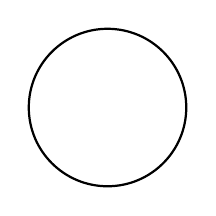
\begin{tikzpicture}[thick]
  \draw (0,0) circle [radius=1cm];
\end{tikzpicture}  
\end{frame}

\begin{frame}
  \centering
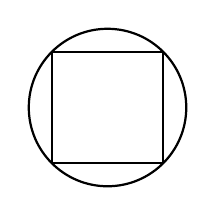
\begin{tikzpicture}[thick]
  \draw (0,0) circle [radius=1cm];
  \draw (45:1cm) rectangle (225:1cm);
\end{tikzpicture}  
\end{frame}

\begin{frame}
  \centering
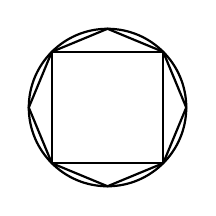
\begin{tikzpicture}[thick]
  \draw (0,0) circle [radius=1cm];
  \draw (45:1cm) rectangle (225:1cm);
  \draw (0:1cm) -- (45:1cm) -- (90:1cm) -- (135:1cm) -- (180:1cm) -- (225:1cm) -- (270:1cm) -- (315:1cm) -- (0:1cm);
\end{tikzpicture}  
\end{frame}

\begin{frame}
  \centering
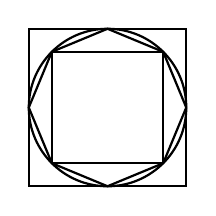
\begin{tikzpicture}[thick]
  \draw (0,0) circle [radius=1cm];
  \draw (45:1cm) rectangle (225:1cm);
  \draw (0:1cm) -- (45:1cm) -- (90:1cm) -- (135:1cm) -- (180:1cm) -- (225:1cm) -- (270:1cm) -- (315:1cm) -- (0:1cm);
  \draw (1cm,1cm) rectangle (-1cm,-1cm);  
\end{tikzpicture}  
\end{frame}

\begin{frame}
  \centering
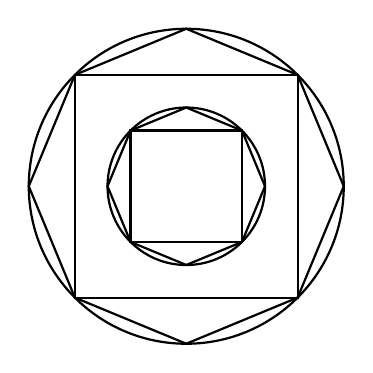
\begin{tikzpicture}[thick]
  \draw (0,0) circle [radius=1cm];
  \draw (45:1cm) rectangle (225:1cm);
  \draw (0:1cm) -- (45:1cm) -- (90:1cm) -- (135:1cm) -- (180:1cm) -- (225:1cm) -- (270:1cm) -- (315:1cm) -- (0:1cm);

  \draw (0,0) circle [radius=2cm];
  \draw (45:2cm) rectangle (225:2cm);
  \draw (0:2cm) -- (45:2cm) -- (90:2cm) -- (135:2cm) -- (180:2cm) -- (225:2cm) -- (270:2cm) -- (315:2cm) -- (0:2cm);
\end{tikzpicture}  
\end{frame}

\begin{frame}
  \centering
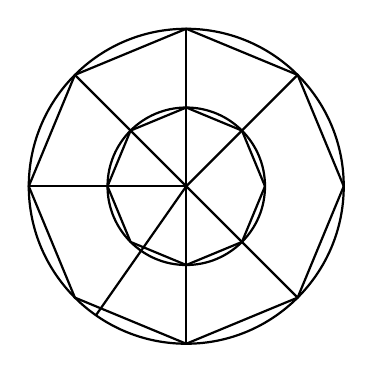
\begin{tikzpicture}[thick]
  \draw (0,0) circle [radius=1cm];
  
  \draw (0:1cm) -- (45:1cm) -- (90:1cm) -- (135:1cm) -- (180:1cm) -- (225:1cm) -- (270:1cm) -- (315:1cm) -- (0:1cm);

  \draw (0,0) circle [radius=2cm];
  \draw (0:2cm) -- (45:2cm) -- (90:2cm) -- (135:2cm) -- (180:2cm) -- (225:2cm) -- (270:2cm) -- (315:2cm) -- (0:2cm);
  \draw (0,0) -- (45:2cm);
  \draw (0,0) -- (90:2cm);
  \draw (0,0) -- (135:2cm);
  \draw (0,0) -- (180:2cm);
  \draw (0,0) -- (235:2cm);
  \draw (0,0) -- (270:2cm);
  \draw (0,0) -- (315:2cm);
  
\end{tikzpicture}  
\end{frame}

\begin{frame}  
  \frametitle{习题}
  \begin{Exercise}
  是否存在一个同时不满足自反性、对称性、反对称性、传递性和反自反性的二元关系?    
  \end{Exercise}
  \begin{Exercise}
  实数集上的“小于”关系$<$是否是反自反的?集合$X$的幂集$2^X$上的“真包含”
  关系$\subset$是否是反自反的?为什么?    
  \end{Exercise}

  \begin{Exercise}
  下列说法是否正确?若正确,请给出证明;若不正确,请说明理由。
  
  1)设$R$为集合$X$上的反自反的和传递的二元关系,则$R$为反对称的二元关系。
  
  2)设$R$为集合$X$上的对称的和传递的二元关系,则$R$为自反的二元关系。    
  \end{Exercise}
\end{frame}
\begin{frame}  
  \frametitle{习题}

  \begin{Exercise}
  设$X = \{1,2,3\}$, $Y = \{1,2\}$,$S = \{f|f:X \to Y\}$。$S$上的二元关系$\cong$定义如下:$\forall f,g\in S$,$f \cong g$当且仅当\[I_m(f) = I_m(g)\]证明$\cong$是$S$上的等价关系,并求出等价类之集。    
  \end{Exercise}
  \begin{Exercise}
  设$X, Y, S$同习题4。$S$上的二元关系$\cong$定义如下:$\forall f,g\in S$,$f \cong g$当且仅当\[f(1) + f(2) + f(3) = g(1) + g(2) + g(3)\]证明$\cong$是$S$上的等价关系,并求出等价类之集。    
  \end{Exercise}

\end{frame}

\begin{frame}
  \frametitle{习题}
 \begin{Exercise}
  设$X, Y, S$同习题4。$S$上的二元关系$\cong$定义如下:$\forall f,g\in S$,$f \cong g$当且仅当\[\{f^{-1}(\{y\}) | y \in Y\} = \{g^{-1}(\{y\})|y \in Y\}\]证明$\cong$是$S$上的等价关系,并求出等价类之集。  
  \end{Exercise}
  \begin{Exercise}
    是否存在一个偏序关系$\leq$,使$(X,\leq)$中有唯一极大元素,但没有最大元素?如
    果有,请给出一个具体例子;如果没有,请证明之。
  \end{Exercise}
  \begin{Exercise}
    令$X=\{a,b,c,d\}$,画出偏序集$(2^X,\subseteq)$的Hasse图。
  \end{Exercise}
\end{frame}
\begin{frame}
  \frametitle{习题}
 \begin{Exercise}
 令$S=\{1,2,\cdots,12\}$,画出偏序集$(S,|)$的Hasse图,其中$|$为整除关系。它有几
 个极大(小)元素?列出这些极大(小)元素。
  \end{Exercise}
  \begin{Exercise}
    偏序集$(X,\leq)$称为有序完备的,当且仅当$X$的每个有上届的非空子集有上确界。
    证明:偏序集$(X,\leq)$为有序完备的当且仅当对$X$的每个有下界的非空子集有下确
    界。
  \end{Exercise}
\end{frame}

\end{CJK*}
\end{document}

%%% Local Variables:
%%% mode: latex
%%% TeX-master: t
%%% End:
